\subsection{Ca sử dụng đổi tên khuôn mặt}

\vspace{0.5cm}

\noindent 
\begin{tabularx}{\linewidth}{| l | X |} 
\hline 
\textbf{Mô tả} & Người dùng đổi tên của nhóm khuôn mặt đã được hệ thống phân loại. \\
\hline 
\textbf{Luồng cơ bản} & 1. Người dùng bấm vào nút đổi tên khuôn mặt. \newline
                       2. Hệ thống hiển thị hộp thoại đổi tên. \newline
                       3. Người dùng nhập tên khuôn mặt mới và submit. \newline
                       5. Hệ thống cập nhật tên và giao diện. \\
\hline
\textbf{Luồng thay thế} & - Tên mới không được trùng với tên nhóm cũ / trống. \\
\hline
\textbf{Tiền điều kiện} & - Người dùng đã đăng nhập vào hệ thống. \newline
                          - Hệ thống đã hoàn thành phân loại khuôn mặt trên ảnh. \\
\hline
\textbf{Hậu điều kiện} & - Người dùng có thể chọn ảnh để xem chi tiết. \newline
                          - Người dùng có thể đổi tên khuôn mặt. \\
\hline 
\textbf{Yêu cầu phi chức năng} & -Hệ thống cập nhật tên khuôn mặt không quá 1s. \\
\hline 
\end{tabularx}

\vspace{0.8cm}

\noindent 
\begin{tabular}{| c | c |}
    \hline
    \textbf{Biểu đồ hoạt động} & \textbf{Quan hệ} \\ 
    \hline
    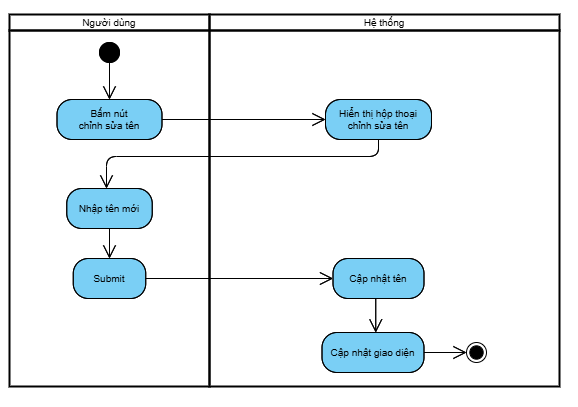
\includegraphics[width=0.6\linewidth]{figures/c3/3-3-12-activity-diagram.png} 
    &  
    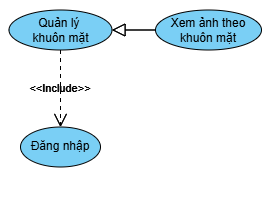
\includegraphics[width=0.35\linewidth]{figures/c3/3-3-12-relationship.png} \\ 
    \hline
\end{tabular}

\begin{figure}[H]
    \centering  
    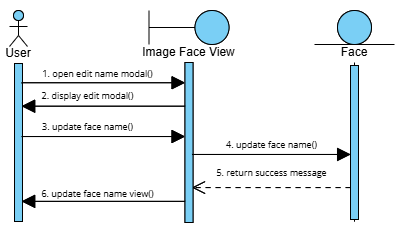
\includegraphics[width=1\textwidth]{figures/c3/3-3-12-sequence-diagram.png}
    \caption{Biểu đồ tuần tự ca sử dụng đổi tên khuôn mặt.}
    \label{fig:3-3-12-sequence-diagram}
\end{figure}